\chapter{Dynaaminen ohjelmointi}

Dynaaminen ohjelmointi on algoritmisuunnittelun tekniikka,
jota voi käyttää kahdenlaisissa tilanteissa:

\begin{itemize}
\item \textbf{Optimiratkaisun etsiminen}: Haluamme etsiä ratkaisun,
joka on jollakin tavalla suurin tai pienin.
\item \textbf{Ratkaisumäärän laskeminen}: Haluamme laskea,
montako erilaista ratkaisua on olemassa.
\end{itemize}

Ideana on muotoilla laskentatehtävä
rekursiivisesti niin, että voimme ratkaista tehtävän
ratkaisemalla ensin osatehtävinä saman tehtävän pienempiä tapauksia.
Aina kun olemme ratkaisseet tietyn osatehtävän,
kirjaamme sen ratkaisun muistiin, minkä ansiosta
pystymme hakemaan ratkaisun tehokkaasti uudestaan,
kun tarvitsemme sitä myöhemmin.

Tässä luvussa tutustumme ensin dynaamisen ohjelmoinnin perusteisiin
käyttäen esimerkkinä tehtävää, jossa haluamme laskea,
monellako tavalla voimme rakentaa tornin palikoista.
Tämän jälkeen käymme läpi joukon muita tehtäviä, jotka esittelevät
dynaamisen ohjelmoinnin mahdollisuuksia.

\section{Perustekniikat}

Aloitamme dynaamiseen ohjelmointiin tutustumisen
seuraavasta tehtävästä:
meillä on palikoita, joiden korkeudet ovat 1, 2 ja 3,
ja haluamme rakentaa niistä tornin, jonka korkeus on $n$.
Jokaista palikkatyyppiä on saatavilla rajattomasti.
Monellako tavalla voimme rakentaa tornin?

\begin{figure}
\center
\begin{tikzpicture}[scale=0.7]
\newcommand\palikka[3]{
\draw (2*#1,#2) rectangle (2*#1+1,#2+#3);
}
%\foreach \i in {0,1,...,6} \draw (2*\i,0) grid (2*\i+1,4);
\palikka{0}{0}{1} \palikka{0}{1}{1} \palikka{0}{2}{1} \palikka{0}{3}{1}
\palikka{1}{0}{1} \palikka{1}{1}{1} \palikka{1}{2}{2}
\palikka{2}{0}{1} \palikka{2}{1}{2} \palikka{2}{3}{1}
\palikka{3}{0}{2} \palikka{3}{2}{1} \palikka{3}{3}{1}
\palikka{4}{0}{2} \palikka{4}{2}{2}
\palikka{5}{0}{1} \palikka{5}{1}{3}
\palikka{6}{0}{3} \palikka{6}{3}{1}
\end{tikzpicture}
\caption{Voimme rakentaa korkeuden 4 tornin 7 tavalla palikoista,
joiden korkeudet ovat 1, 2 ja 3.}
\label{fig:dyntor}
\end{figure}

Kuva \ref{fig:dyntor} näyttää esimerkin, jossa $n=4$.
Tässä esimerkissä meillä on 7 tapaa rakentaa torni palikoista.
Voimme luonnehtia torneja myös summina luvuista 1, 2 ja 3.
Tässä tapauksessa vasen torni vastaa summaa $1+1+1+1$,
seuraava torni vastaa summaa $1+1+2$, jne.

Jos $n$ on pieni, voimme laskea tornien määrän helposti
käymällä läpi kaikki tavat, mutta tornien määrä kasvaa
nopeasti emmekä voi käyttää raakaa voimaa suuremmilla
$n$:n arvoilla.
Seuraavaksi ratkaisemmekin ongelman tehokkaasti
dynaamisen ohjelmoinnin avulla.

\subsection{Rekursiivinen esitys}

Jotta voimme käyttää dynaamista ohjelmointia,
meidän täytyy esittää ongelma rekursiivisesti
niin, että saamme laskettua ongelman ratkaisun
käyttäen osaongelmina pienempiä vastaavia ongelmia.

Tässä tehtävässä meidän on luontevaa määritellä rekursiivinen
funktio $\texttt{tornit}(n)$: monellako tavalla voimme
rakentaa tornin, jonka korkeus on $n$?
Esimerkiksi $\texttt{tornit}(4)=7$, koska tiedämme
esimerkkimme ansiosta,
että voimme rakentaa korkeuden 4 tornin 7 tavalla.

Funktion pienten arvojen laskeminen on helppoa.
Ensinnäkin $\texttt{tornit}(0)=1$, koska voimme
muodostaa tyhjän tornin yhdellä tavalla:
siinä ei ole mitään palikoita.
Sitten $\texttt{tornit}(1)=1$, koska ainoa mahdollisuus
on valita korkeuden 1 palikka,
ja $\texttt{tornit}(2)=2$, koska voimme joko valita
kaksi korkeuden 1 palikkaa tai yhden korkeuden 2 palikan.

\begin{figure}
\center
\begin{tikzpicture}[scale=0.7]
\draw (0,0) rectangle (1,1);
\draw[dashed] (0,1) rectangle (1,4);
\draw (4,0) rectangle (5,2);
\draw[dashed] (4,2) rectangle (5,4);
\draw (8,0) rectangle (9,3);
\draw[dashed] (8,3) rectangle (9,4);
\draw [decorate,decoration={brace,amplitude=4pt},xshift=0.2cm] (1,4) -- (1,1) node [midway,right,xshift=.1cm] {$n-1$};
\draw [decorate,decoration={brace,amplitude=4pt},xshift=0.2cm] (5,4) -- (5,2) node [midway,right,xshift=.1cm] {$n-2$};
\draw [decorate,decoration={brace,amplitude=4pt},xshift=0.2cm] (9,4) -- (9,3) node [midway,right,xshift=.1cm] {$n-3$};
\end{tikzpicture}
\caption{Rekursiivinen idea: kun alamme rakentaa tornia, voimme laittaa pohjalle
korkeuden 1, 2 tai 3 palikan.}
\label{fig:dynrek}
\end{figure}


Kuinka voisimme sitten laskea funktion arvon yleisessä tapauksessa,
kun tornin korkeus on $n$?
Tässä voimme miettiä, kuinka tornin rakentaminen alkaa.
Meillä on kolme mahdollisuutta: voimme laittaa ensin palikan
korkeutta 1, 2 tai 3.
Jos valitsemme korkeuden 1 palikan, meidän täytyy rakentaa
sen päälle korkeuden $n-1$ torni.
Vastaavasti jos valitsemme korkeuden 2 tai 3 palikan,
meidän täytyy rakentaa sen päälle torni,
jonka korkeus on $n-2$ tai $n-3$.
Kuva \ref{fig:dynrek} havainnollistaa tämän idean.

Niinpä voimme laskea tornien määrän rekursiivisesti kaavalla
\[
\texttt{tornit}(n) = \texttt{tornit}(n-3)+\texttt{tornit}(n-2)+\texttt{tornit}(n-1),
\]
kun $n \ge 3$.
Esimerkiksi voimme laskea
\[
\texttt{tornit}(3) = \texttt{tornit}(0)+\texttt{tornit}(1)+\texttt{tornit}(2)=4
\]
ja
\[
\texttt{tornit}(4) = \texttt{tornit}(1)+\texttt{tornit}(2)+\texttt{tornit}(3)=7,
\]
jolloin olemme saaneet laskettua esimerkkitapaustamme vastaavasti,
että voimme rakentaa korkeuden 4 tornin 7 tavalla.

\begin{table}
\center
\begin{tabular}{rrr}
korkeus $n$ & $\texttt{tornit}(n)$ \\
\hline
0 & 1 \\
1 & 1 \\
2 & 2 \\
3 & 4 \\
4 & 7 \\
5 & 13 \\
6 & 24 \\
7 & 44 \\
8 & 81 \\
9 & 149 \\
\end{tabular}
\caption{Tornien määrät, kun korkeus $n$ on $0,1,\dots,9$.}
\label{tab:dyntor}
\end{table}

Taulukko \ref{tab:dyntor} näyttää yhteenvedon funktion
$\texttt{tornit}(n)$ arvoista, kun $n=0,1,\dots,9$.
Kuten taulukosta voi huomata, funktion arvo kasvaa nopeasti:
se lähes kaksinkertaistuu joka askeleella.
Kun $n$ on suuri,
meillä onkin valtavasti mahdollisuuksia tornin rakentamiseen.

\subsection{Tehokas toteutus}

Nyt kun olemme saaneet aikaan rekursiivisen funktion,
voimme toteuttaa sen ohjelmoimalla seuraavasti:

\begin{code}
long tornit(int n) {
    if (n == 0) return 1;
    if (n == 1) return 1;
    if (n == 2) return 2;
    return tornit(n-3)+tornit(n-2)+tornit(n-1);
}
\end{code}

Tämä on toimiva ratkaisu, mutta siinä on yksi ongelma:
funktion arvon laskeminen vie kauan aikaa, jos $n$ on
vähänkin suurempi.
Käytännössä laskenta alkaa hidastua parametrin $n=30$ tienoilla.
Esimerkiksi arvon $\texttt{tornit}(40)$ laskeminen vie aikaa
jo useita minuutteja, ja voimme arvioida, että
arvon $\texttt{tornit}(50)$ laskeminen veisi aikaa noin vuorokauden.

Syynä laskennan hitauteen on, että metodia $\texttt{tornit}$
kutsutaan uudestaan ja uudestaan samoilla parametreilla
ja tornien määrä lasketaan loppujen lopuksi summana
luvuista 1 ja 2 pohjatapauksista.
Niinpä kun tornien määrä on suuri,
laskenta on tuomittu viemään kauan aikaa.
Voimme kuitenkin selviytyä ongelmasta toteuttamalla
laskennan hieman toisella tavalla.

Tässä astuu kuvaan dynaamisen ohjelmoinnin keskeinen idea:
laskemme funktion arvon kullekin parametrille vain kerran
ja tallennamme tulokset taulukkoon myöhempää käyttöä varten.
Tätä varten luomme taulukon $\texttt{tornit}$,
jossa kohtaan $\texttt{tornit}[i]$ tallennetaan funktion
arvo $\texttt{tornit}(i)$.
Kun haluamme laskea korkeuden $n$ tornien määrän,
täytämme taulukon kohdat $0,1,\dots,n$.
Seuraava koodi toteuttaa laskennan:

\begin{code}
long[] tornit = new long[n+1];
tornit[0] = 1;
tornit[1] = 1;
tornit[2] = 2;
for (int i = 3; i <= n; i++) {
    tornit[i] = tornit[i-3]+tornit[i-2]+tornit[i-1];
}
\end{code}

Koodin suorituksen jälkeen taulukon arvo $\texttt{tornit}[n]$
kertoo meille, monellako tavalla voimme rakentaa
korkeuden $n$ tornin.

Tämän toteutuksen etuna on, että se on huomattavasti
nopeampi kuin rekursiivinen metodi.
Koska koodissa on vain yksi for-silmukka, se vie aikaa
vain $O(n)$, eli voimme käsitellä tehokkaasti myös
suuria $n$:n arvoja.
Esimerkiksi voimme nyt laskea salamannopeasti, että
\[
\texttt{tornit}(50) = 10562230626642,
\]
eli meillä on yli 10562 miljardia tapaa rakentaa korkeuden 50 torni.

\section{Esimerkkejä}

Nyt olemme käyneet läpi dynaamisen ohjelmoinnin perustekniikat
ja on aika ottaa käsittelyyn lisää tehtäviä,
jotka opettavat meille lisää dynaamisesta ohjelmoinnista.

Dynaamista ohjelmointia voi käyttää aina silloin,
kun voimme esittää tilanteen rekursiivisena funktiona,
jonka eri parametrien määrä on niin pieni, että voimme
tallentaa muistiin funktion arvot kaikilla parametreilla.
Vaikeutena on usein keksiä, mikä on hyvä rekursiivinen
muotoilu tehtävälle.

\subsection{Pisin nouseva alijono}

Ensimmäinen tehtävämme on laskea, kuinka pitkä on
$n$ lukua sisältävän taulukon \emph{pisin nouseva alijono}.
Tämä tarkoittaa, että meidän tulee valita taulukosta
mahdollisimman pitkä jono alkioita niin,
että seuraava alkio on aina edellistä suurempi.
Kuvassa \ref{fig:pisnou} on esimerkki taulukosta,
jonka pisin nouseva alijono on pituudeltaan 4.

\begin{figure}
\center
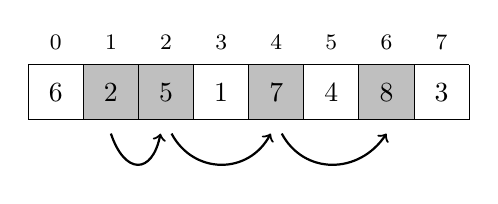
\begin{tikzpicture}[scale=0.7]
\fill[color=lightgray] (1,0) rectangle (2,1);
\fill[color=lightgray] (2,0) rectangle (3,1);
\fill[color=lightgray] (4,0) rectangle (5,1);
\fill[color=lightgray] (6,0) rectangle (7,1);
\draw (0,0) grid (8,1);
\node at (0.5,0.5) {$6$};
\node at (1.5,0.5) {$2$};
\node at (2.5,0.5) {$5$};
\node at (3.5,0.5) {$1$};
\node at (4.5,0.5) {$7$};
\node at (5.5,0.5) {$4$};
\node at (6.5,0.5) {$8$};
\node at (7.5,0.5) {$3$};
\draw[thick,->] (1.5,-0.25) .. controls (1.75,-1.00) and (2.25,-1.00) .. (2.4,-0.25);
\draw[thick,->] (2.6,-0.25) .. controls (3.0,-1.00) and (4.0,-1.00) .. (4.4,-0.25);
\draw[thick,->] (4.6,-0.25) .. controls (5.0,-1.00) and (6.0,-1.00) .. (6.5,-0.25);
\footnotesize
\node at (0.5,1.4) {$0$};
\node at (1.5,1.4) {$1$};
\node at (2.5,1.4) {$2$};
\node at (3.5,1.4) {$3$};
\node at (4.5,1.4) {$4$};
\node at (5.5,1.4) {$5$};
\node at (6.5,1.4) {$6$};
\node at (7.5,1.4) {$7$};
\end{tikzpicture}
\caption{Taulukon pisin nouseva alijono on $[2,5,7,8]$.}
\label{fig:pisnou}
\end{figure}

Voimme lähestyä tehtävää laskemalla jokaiselle taulukon
kohdalle $x=0,1,\dots,n-1$ arvon $\texttt{pisin}(x)$:
kuinka pitkä on pisin nouseva alijono, joka päättyy tähän kohtaan.
Kun olemme laskeneet kaikki nämä arvot, suurin arvoista kertoo,
kuinka pitkä on pisin nouseva alijono koko taulukossa.
Esimerkiksi kuvan \ref{fig:pisnou} taulukossa $\texttt{pisin}(6)=4$,
koska kohdassa $6$ pisin nouseva alijono on pituudeltaan $4$.

Millainen on sitten pisin kohtaan $x$ päättyvä alijono?
Yksi mahdollisuus on, että alijonossa on vain yksi alkio,
jolloin $\texttt{pisin}(x)=1$.
Jos kuitenkin alijonossa on useampia alkioita,
voimme käydä läpi vaihtoehdot, missä kohdassa on alijonon
toiseksi viimeinen alkio.
Meidän täytyy siis tarkastella kohtia $k$, joille pätee $k<x$
ja joiden alkiot ovat pienempiä kuin kohdan $x$ alkio.
Jokaisessa tällaisessa tapauksessa voimme muodostaa alijonon,
jossa on ensin pisin kohtaan $k$ päättyvä alijono ja
sitten vielä kohdan $x$ alkio.
Tuloksena olevan alijonon pituus on $\texttt{pituus}(k)+1$.
Jokin tällainen alijono on varmasti pisin kohtaan $x$ päättyvä alijono.

Seuraava koodi laskee jokaiseen kohtaan $x=0,1,\dots,n-1$
pisimmän kohtaan päättyvän alijonon pituuden yllä kuvattua
ideaa käyttäen.
Koodi olettaa, että taulukon sisältö on taulukossa \texttt{taulu},
ja se muodostaa taulukon \texttt{pisin}, jossa on pisimpien
alijonojen pituudet.
Koodin suoritus vie aikaa $O(n^2)$, koska siinä on kaksi sisäkkäistä silmukkaa.

\begin{code}
for (int i = 0; i < n; i++) {
    pisin[i] = 1;
    for (int j = 0; j < i; j++) {
        if (taulu[j] < taulu[i]) {
            pisin[i] = max(pisin[i],pisin[j]+1);
        }
    }
}
\end{code}

\subsection{Repunpakkaus}

\subsection{Reitti ruudukossa}
